\zexternaldocument{inleiding}
\zexternaldocument{analyse}

\chapter{Evaluatie}
\label{sec:evaluatie}
Om de impact van de verschillende heuristieken te meten volgt nu een overzicht van de testresultaten.
Voor het merendeel van de testen is een simulator gebruikt.
Sectie \ref{sec:simulator} legt uit waarom een simulator gebruikt wordt in plaats van IMP zelf, en hoe deze werkt.

De daarop volgende secties bespreken de resultaten van elke heuristiek. 
De algemene verwachting is dat het gebruik van heuristieken het aantal deployment runs reduceert en zo ook de totale uitroltijd.
Deze optimalisatie kost wel extra verwerkingstijd (de uitvoering van de verschillende heuristieken) maar deze is normaal gezien te verwaarlozen ten opzichte van het volledige uitrolproces.\todo{meten} 

\section{Simulator}
\label{sec:simulator}
Er zijn twee belangrijke voordelen aan het gebruiken van een simulator.
Ten eerste is de uitroltijd evenredig met de grootte van het model.
Zelfs met het gebruik van heuristieken om het aantal deployment runs te minimaliseren blijft een significant deel van het proces gespendeerd aan bijvoorbeeld het downloaden van pakketten. 
Ten tweede laat een simulator toe modellen met honderden machines uit te rollen op \'e\'en enkele pc.

De simulator bootst een systeem na dat Fedora 18 draait en gebruik maakt van de yum pakket manager.

\subsection{Uitwerking}
\label{simulator:uitwerking}
Het proces begint nog altijd bij IMP zelf.
Als de gebruiker de optie ``-j'' meegeeft compileert IMP het model volledig maar in plaats van het dan uit te rollen, schrijft hij het weg in een JSON bestand.
De simulator gebruikt dat bestand als invoer om het uitrolproces te simuleren.
Het resultaat van een simulatierun is een sqlite-database waarin alle hosts en hun resources vermeld staan (de deployment database genoemd).
Om de simulatie zo waarheidsgetrouw mogelijk te maken houdt de simulator rekening met volgende aspecten van het uitrolproces:

\begin{itemize}
  \item Bestanden en mappen kunnen niet aangemaakt worden voordat de bovenliggende map bestaat
  \item Services kunnen niet gestart worden voordat het bijhorende pakket en bestanden aanwezig zijn
  \item Resources worden pas aangemaakt als hun afhankelijkheden voldaan zijn
\end{itemize}

De simulator maakt gebruik van twee externe informatiebronnen: een lijst van standaard mappen die aanwezig zijn na een nieuwe Fedora installatie en de repository data van verschillende yum repositories.
Beide helpen bij het correct uitrollen van de resources.

Het uitrollen van een file gaat als volgt:
\begin{lstlisting}[showstringspaces=false]
def deploy_file(file):
  #Check if parent folder exists already
  if file in std_filesystem or file in deployment_database:
    deployment_database.write(file)
  else:
    error('Parent folder doesn't exist!')
\end{lstlisting}

Het uitrollen van een service gaat als volgt: 
\begin{lstlisting}
def deploy_service(srv):
  #Check if required files have been deployed
  requirements = repodata_database.execute('select * from pkgdata where name like srv.name')
  if all([req in deployment_database for req in requirements]):
    deployment_database.write(srv)
  else:
    error('Not all required resources were deployed!')
\end{lstlisting}

Het uitrollen van een pakket gaat als volgt: 
\begin{lstlisting}
def deploy_package(pkg):
  pkg_files = repodata_database.execute('select * from pkgdata where name like pkg.name') 
  foreach file in pkg_files:
    deployment_database.write(file)
\end{lstlisting}
We gaan er van uit dat fouten bij het uitrollen van een pakket de verantwoordelijkheid zijn van de package manager (hier yum), niet de CMS.

\todo{Verschil in uitroltijd simulator/IMP?}
\todo{Besluit sectie}

\section{Afhankelijkheden tussen bestanden en mappen}
\label{sec:bestanden_en_mappen_eval}
Aangezien een bestand niet kan gecre\"eerd worden zonder zijn bovenliggende map voegt deze heuristiek automatisch de afhankelijkheid tussen beide toe aan het model.

Aangezien mappen altijd kunnen gecre\"eerd worden zijn er maximaal twee deployment runs nodig als er geen heuristiek gebruikt wordt.
Bij gebruik van de heuristiek moet er exact \'e\'en uitgerold worden.
De verwachting is dat het uitrollen met gebruik van de heuristiek dan ook ongeveer half zo lang duurt.

Figuur \ref{fig:file_dir_times} toont de resultaten van deze test.
Elk datapunt is het gemiddelde van 30 runs, uitgevoerd op een virtuele machine met twee cores van 2Ghz en 2GB RAM ter beschikking.
Het model bestaat iedere keer uit vast aantal bestanden en mappen, \'e\'en bestand per map.
\begin{figure}[h]
    \begin{center}
    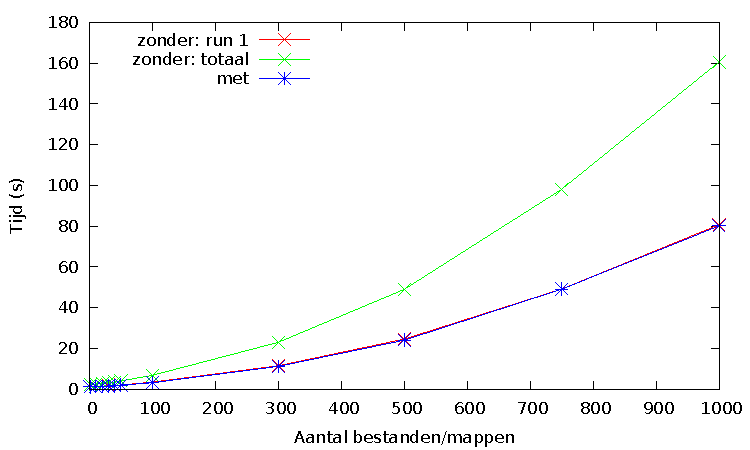
\includegraphics[width=0.8\textwidth]{images/file_dir_times.pdf}
    \caption{Testresultaten bij het uitrollen van een stijgend aantal bestanden en mappen, met en zonder gebruik van de heuristiek}
    \label{fig:file_dir_times}
    \end{center}
\end{figure}

De verwachtingen zijn volledig ingelost: zonder heuristiek zijn er twee deployment runs nodig, met heuristiek slechts \'e\'en.
Dit weerspiegelt zich in de gehalveerde uitroltijd.

\section{Afhankelijkheden tussen services, pakketten en configuratiebestanden}
\label{sec:stacks_eval}
De specificatie van een service in het configuratiemodel gaat vaak gepaard met de pakket en de configuratiebestanden die die service nodig heeft.
Deze combinatie van resources wordt een stack genoemd.
Aangezien de service niet correct werkt zonder de aanwezigheid van het pakket en de configuratiebestanden voegt deze heuristiek de gepaste vereisten toe aan het model.


Voor deze test moest IMP 30 keer de NTP service uitrollen op een testmachine.
NTP bestaat uit \'e\'en pakket, \'e\'en configuratiebestand en \'e\'en service. 
In het slechtste geval zijn er normaal gezien dus drie deployment runs nodig om de service correct werkende te krijgen.
Als de correcte afhankelijkheden worden opgesteld is er slechts \'e\'en run nodig.
De testresultaten zijn te vinden in tabel \ref{table:service_package_dep}.

\begin{table}
  \begin{center}
  \label{table:service_package_dep}
  \begin{tabular}{ r | c | c }
            & tijd(s)   & gemiddeld aantal runs nodig \\ \hline
    zonder  & 3.21      & 2.0 \\ \hline
    met     & 2.21      & 1 \\
  \end{tabular}
  \caption{Meetresultaten}
  \end{center}
\end{table}
%specifieke resultaten:
%zonder
%Avg time: 3.212880388398965
%Deployments avg: 2.0
%met: Avg time: 2.2067235755423704
%deps toegevoegd: 3

De resultaten van de test zijn zoals verwacht: dankzij de heuristiek is maar \'e\'en deployment run nodig.

\section{Relaties en afhankelijkheden tussen hoog-niveau concepten}
Door het omzetten van relaties naar afhankelijkheden kan het nodige aantal deployment runs gereduceerd worden.

\section{Use cases}

\subsection{Document processing}

\todo{Uitleg geven over use case}

\todo{Dit is eigenlijk geen uitleg van de toepassing van de heuristieken op de use case, meer een uitleg/test van de heuristieken}
In afbeelding \ref{fig:reqs_doc} is te zien hoeveel vereisten elke heuristiek toevoegen.
De heuristiek die de bovenliggende map toevoegt aan de vereisten van een map of bestand wordt altijd uitgevoerd.
Deze heuristiek beschouwen we namelijk als fundamenteel: de vereisten die ze toevoegd zijn sowieso juist, terwijl sommige vereisten die door andere heuristieken worden toegevoegd mogelijks overbodig zijn. 

De verwachting is dat sommige heuristieken zullen overlappen, bijvoorbeeld ``stack'' en ``name''. 
Resources binnen dezelfde stack hebben namelijk vaak een gelijkaardige naam. 

\begin{figure}[h]
    \begin{center}
    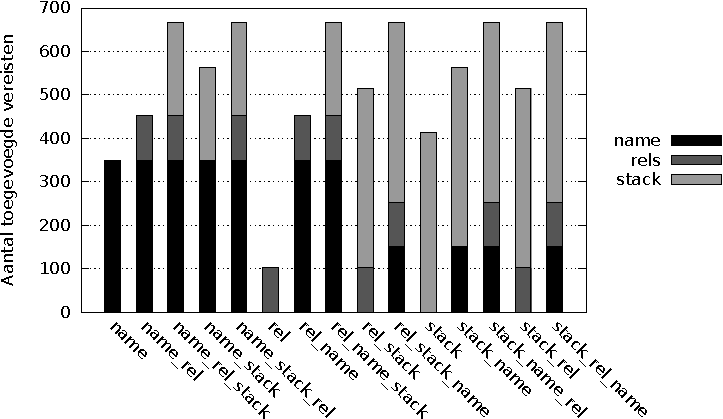
\includegraphics[width=0.8\textwidth]{images/reqs_doc.pdf}
    \caption{Aantal toegevoegde vereisten voor elke combinatie van heuristieken in de document processing use case}
    \label{fig:reqs_doc}
    \end{center}
\end{figure}

Als een bepaalde heuristiek eerst toegepast wordt kan hij al zijn vereisten toevoegen.
Daaropvolgende heuristieken zullen enkel het deel van hun vereisten toevoegen die nog niet deel uitmaken van het model.
Ongeacht de volgorde zal een combinatie heuristieken altijd dezelfde set vereisten toevoegen.

In afbeelding \ref{fig:time_runs_doc} is te zien welke impact de toegevoegde vereisten hebben op het uitrolproces.

\begin{figure}[h]
    \begin{center}
    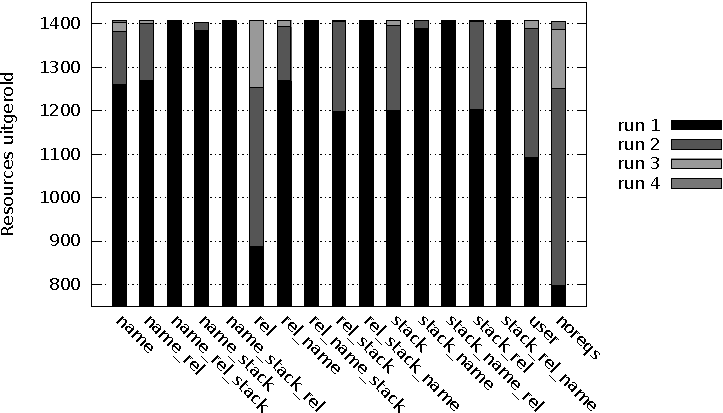
\includegraphics[width=0.8\textwidth]{images/time_runs_doc.pdf}
    \caption{Gemiddelde aantal uitgerolde resources per deployment run voor elke combinate van heuristieken in de document processing use case}
    \label{fig:time_runs_doc}
    \end{center}
\end{figure}

De resultaten bevestigen onze aanname dat het toevoegen van vereisten kan leiden tot een daling in het aantal deployment runs.
Elke combinatie van de drie heuristieken leidt zelfs tot een ``one-shot'' uitrolproces waarin in \'e\'en keer het volledige model correct uitgerold wordt.

\subsection{MongoDB}

MongoDB is een van de meer bekende NoSQL databases.
Een volledige configuratie bestaat uit verschillende services die elkaar ondersteunen.
Figuur \ref{fig:mongodb_architecture} geeft een schematische voorstelling van een dergelijke set-up. \todo{cite}

\begin{figure}[h]
    \begin{center}
    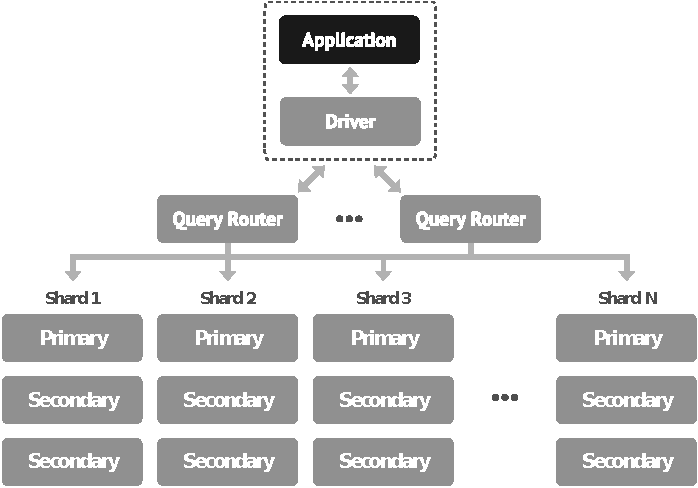
\includegraphics[width=0.8\textwidth]{images/mongodb_architecture.pdf}
    \caption{Architectuur van de MongoDB database}
    \label{fig:mongodb_architecture}
    \end{center}
\end{figure}

In het model dat Thomas Uyttendaele opgesteld heeft \todo{cite} krijgen de onderdelen de volgende namen:

\begin{table}[h!]
  \begin{center}
  \begin{tabular}{c | c}
  Query Router  & AccessServer \\ \hline
  Primary       & ReplicaSetController \\ \hline
  Secondary     & Node \\ 
  \end{tabular}
  \end{center}
\end{table}

De onderdelen zullen pas correct kunnen samenwerken als ze in de juiste volgorde worden opgestart.
Het is dus weerom \todo{Vroeger vermelden dat het van groot belang is dat het model compleet is} van groot belang dat alle afhankelijkheden in het model
vermeld worden.

Voor de volgende resultaten werd een instantie van MongoDB uitgerold met vijf nodes, verdeeld in twee replicasets van twee en drie nodes elk.
Drie nodes nemen ook de rol van Query Router op zich.
Figuur \ref{fig:reqs_mongo} toont de vereisten die elke combinatie van heuristieken toevoegt.

\begin{figure}[h]
    \begin{center}
    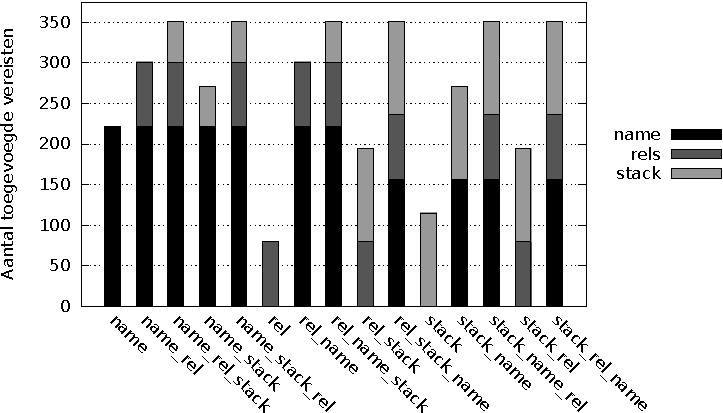
\includegraphics[width=0.8\textwidth]{images/reqs_mongo.pdf}
    \caption{Aantal toegevoegde vereisten voor elke combinatie van heuristieken bij MongoDB}
    \label{fig:reqs_mongo}
    \end{center}
\end{figure}

Figuur \ref{fig:time_runs_mongo} toont hoeveel deployment runs nodig zijn om een volledig werkende MongoDB database te bekomen, en hoeveel resources er
per run gedeployed worden.

\begin{figure}[h]
    \begin{center}
    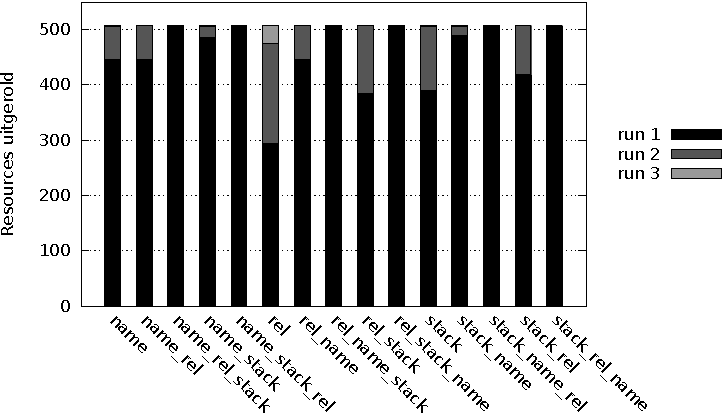
\includegraphics[width=0.8\textwidth]{images/time_runs_mongo.pdf}
    \caption{Gemiddelde aantal uitgerolde resources per deployment run voor elke combinate van heuristieken bij MongoDB}
    \label{fig:time_runs_mongo}
    \end{center}
\end{figure}
